\section{Method}
The general idea is to generate the medial axis transform and round the distance measures,
such that an exact integer beads will fit the polygon there
so that there is never a gap region left over in the middle of the polygon.

We round to integer multiples of half the nozzle width so as to allow single-bead segments, rather than only having polygonal insets.

\begin{figure}
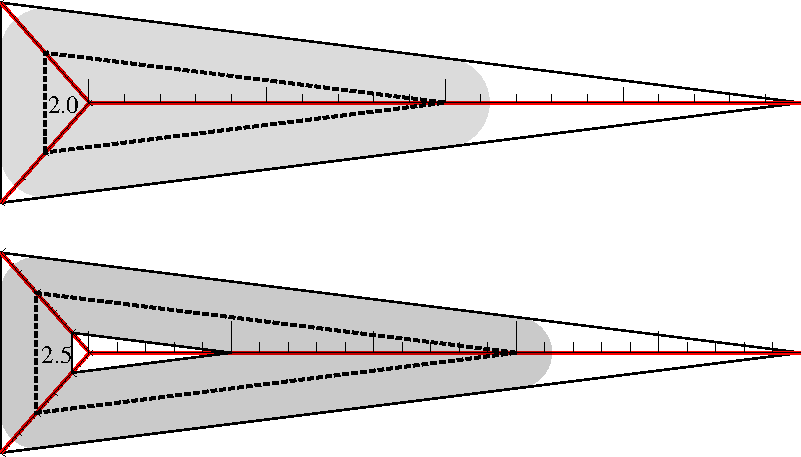
\includegraphics[width=\columnwidth]{sources/method/rounded_vs_unrounded.pdf}
\caption{Toolpaths employing dist rounding vs without.}
\label{rounded_vs_unrounded}
\end{figure}


\begin{figure}
\begin{subfigure}{0.45\columnwidth}
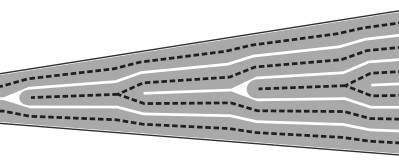
\includegraphics[width=\columnwidth]{sources/method/single_bead_strategy.jpg}
\caption{Overview}
\label{single_bead_strategy_overview}
\end{subfigure}
\begin{subfigure}{0.45\columnwidth}
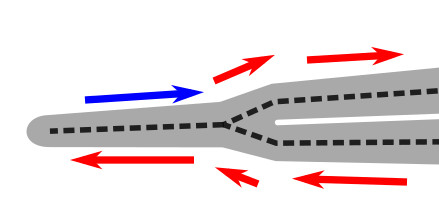
\includegraphics[width=\columnwidth]{sources/method/single_bead_strategy_order.jpg}
\caption{Travel order}s
\end{subfigure}
\caption{We can do single-bead segments. Blue is travel move.}
\label{single_bead_strategy}
\end{figure}

\subsection{Method Overview}
The global idea is that we locally decide on the number of beads everywhere in the input shape, then apply a beading strategy to determine the widths of the beads and then generate the toolpath locations and widths from this.
We decide on a bead count at locations which lie in the middle of the shape in some sense to be defined.
The beading strategy then gives us the beading widths and locations in between those center locations and the outline.
These beadings are then used to generate the toolpath junctions, which are connected together to form the extrusion toolpaths with varying width.

\begin{enumerate}
\item Compute a skeletonization of the outline shape based on the Voronoi diagram.
\item Use a significance measure to mark portions of the skeleton which lie in the center.
\item Determine the bead count values in the marked regions and handle transitions in bead count values.
\item Generate ticks along non-marked bones of the skeleton and connect the ticks together to extract the toolpaths.
\end{enumerate}


\hl{Idea: generate only outer 3 walls, except in marked regions where the distance $R < 5 \win$, so as to prevent jagged infill lines.}
\Cref{wedge_and_infill}

\hl{Filter beading number in order to prevent regions with a lot of back and forth transitions.}

\subsection{Terminology}
For an explanation of the terms used, see \cref{legend}.

\begin{figure}
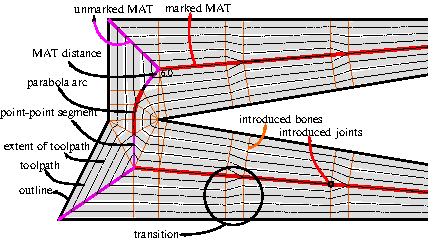
\includegraphics[width=\columnwidth]{sources/method/legend_double_wedge_example.pdf}
\caption{Explanation of terms.}
\label{legend}
\end{figure}



\hl{We need consistent terminology and symbols which adhere to standards in literature.}
The following synonym groups are used here which are not yet checked with existing literature':
\begin{itemize}
\item bones, medial axis segments, arms, fingers, ribs
\item joints, ticks, medial axis vertices, locations
\item MAT distance measure
\end{itemize}


Based on the straight skeleton naming, I would like to introduce a new consistent terminology:
\begin{itemize}
\item marked medial axis segment: vertebra
\item marked medial axis: spine
\item non-marked medial axis segment: arm
\item any medial axis segment: bone
\item bone introduced to the medial axis: rib
\item medial axis vert: joint
\item location of an insets along a bone: tick? locus?
\end{itemize}












\subsection{Beading strategy}
First we determine how we should fill a 	polygon with constant width with a number of beads.
We want to fit an exact whole number of beads in order to prevent a gap being generated.
We consider only half of the polygon, because our beading strategy should be symmetrical.

We define a beading strategy as the following set:
$$
\left\{ b(d), p(n), W(n, d), L(n, d), t, \alpha_{\text{max}} \right\}
$$
where
$b(d)$ gives the optimal bead count to cover a total distance of $d$,
$p(n)$ gives the optimal total distance of a given bead count $n$,
$W(n, d)$ gives the sequence of bead widths to cover a distance $d$ using $n$ beads,
$L(n, d)$ gives the sequence of toolpath positions as distances from the outline to cover a distance $d$ using $n$ beads,
$t$ is the length of transitions within which we switch to a different number of beads
and
$\alpha_{\text{max}}$ is the limit bisector angle of the significance measure.


We call a distance $d$ `prefered' when $d = p(b(d))$
For our method we require the inverse $b^{-1}(n)$ which gives the smallest $d$ for which $b(d) = n$.

The following restrictions hold:
\begin{itemize}
\item $b(d) \geq 0, W(n,d) > 0, L(n, d) \geq 0, t \geq 0$
\item $120\degree < \alpha_{\text{max}} \leq 180\degree$
\item $W$ is symetric: $W(n, d)_i = W(n, d)_{n-i-1}$
\item $L$ is symmetric in $d$: $L(n, d)_i = d - L(n, d)_{n-i-1}$
\item $p$ is within the range of optimal: $b^{-1}(n) < p(n) < b^{-1}(n + 1)$
%\item $b \left( p(n) \right) = n$ % follows from the above!
\item $b$ is monotonic: $ b(d) \leq b(d + \epsilon)$
\item $W_n$ is monotonic and continuous at each bead index $n$ for constant bead count $c$: $0 \leq \frac{\partial W(c, d)_n}{\partial d} < \infty$.
\item $t$ is viable: $\forall i \in \mathbb{N} : t < \left( p(i + 1) - p(i) \right) /{2 \cos \alpha_\text{max}}$
\end{itemize}

The angle requirement ensures that there is never a 3-way junction of significant bones.

By applying the beading strategy to a skeleton location $v$ and a predetermined bead count $n$ we get a beading, which is defined as the following set:
$$
\left\{ d, w_i, l_i  \right\}
$$
where
$d = 2 R(v)$ is the total distance associated with $v$,
$w_i$ is the bead width of the bead with index $i$
end
$l_i$ is the distance of the toolpath location of bead $i$ from the outline.






\subsubsection{Proposed optimal beading strategy}
@Readers: you can skip reading this section for now.
\todo{This section is about some optimal strategy which hasn't been fully developed (yet?).}
\todo{This section still formules the beading strategy in terms of radius instead of diameter, which halves the $n$ values.}

We need a function $W$ from a given radial distance $R(v)$ to a number of beads and their widths.
These widths depend on the following parameters:
\begin{description}
\item[$\wmin$] the minimum possible bead width
\item[$\wmax$] the maximum possible bead width
\item[$\wout$] the preferred bead width of the outer inset
\item[$\win$] the preferred bead width of the other insets
\end{description}

The function $W$ needs to be able to deal with a range which is considerably shorter than $[\wmin, 2\wmin]$, even so short as to accomodate just $[\win,\win]$ only.
The function needs to be such that we never overshoot the radial distance $R(v)$, because that would affect the dimensional accuracy.
Any distance left over which cannot be filled given the range $[\wmin, \wmax]$ should be placed on the inside near the MAT.

We define $W(d)$ as a sequence of bead widths.
The length of that sequence is $b(d)$.
For example: with $\win = \SI{0.4}{\milli\meter}$ we could have $b(1.05) = 2.5$ and $W(1.05) = (0.4, 0.4, 0.5)$.
The last number is the innermost bead width if there is a singleton bead along the medial axis; only half of that bead spans along a radial distance.

The function $b$ should adhere to several criteria:
\begin{itemize}
\item $b \left( \frac12 n\win \right) = \frac12 n$ for integer $n$
%\item $b$ is monotonic
%the item below follows from the two above
% \item between a location with radial distance $R(v) \in [\frac12 n\win, \frac12 (n+1)\win]$ (for integer $n$) there is only one transition to a different number of beads
\item $ 0 \leq b(d) \leq d / w_\text{min} $
%\item the width $W(c, d)_n$ of each bead $n$ increases monotonically and gradually in regions with constant bead count $c$: $0 \leq \frac{\partial W(c, d)_n}{\partial d} < \infty$.
\end{itemize}


For our application we define a $W$ adhereing to the following aditional constraints in order of priority:
\begin{itemize}
\item Minimize unfilled area
\item Try to get the outer bead width $W_1$ as close as possible to $\wout$
\item Have the rest of the $W_n$ the same width
\item at transition regions decide between $n$ and $n+1$ beads using the Loss fuction scheme below
\item From a $d$ for which $b(d) = 3$ we don't consider fractional $b(d)$ anymore; we don't allow singleton beads along the medial axis.
\hl{Perhaps we should disallow this because that would require a different transition length}
\end{itemize}

\iffalse
\begin{align}
W(d)_1 = 
  \begin{cases} 
%  \infty & \text{if } w < w_\text{min} \\
   \wout & \text{if } d \geq \wout + \wmin \\
   w - \wmin  & \text{if } 2\wmin  \leq d < \wout + \wmin
  \end{cases}
\end{align}
\fi

%\subsubsection{Optimal beading strategy}
%We could decide on a beading strategy based on some loss function $L$ defined on each line width.

\begin{align}
L(w_1) &= 
  \begin{cases} 
%  \infty & \text{if } w < w_\text{min} \\
   (w - \wout) / (\wmax - \wout) & \text{if } w > \wout\\
   (\wout - w) / (\wout - \wmin)       & \text{otherwise}
  \end{cases}
  \\
L(w_n) &= 
  \begin{cases} 
%  \infty & \text{if } w < w_\text{min} \\
   (w - \win) / (\wmax - \win) & \text{if } w > \win\\
   (\win - w) / (\win - \wmin)       & \text{otherwise}
  \end{cases}
\\
L(W(d)) &= \left(b(d) - \lfloor b(d) \rfloor \right) L \left( W(d)_{\lceil b(d) \rceil} \right)  +  \sum_{n=1}^{n=\lfloor b(d) \rfloor} L( W(d)_n )
\end{align}

(Singular beads are counted only half.)
Together these prioritized constraints uniquely define a single $W$, depending on $\wmin, \wmax, \wout,\win$.
An example is given in \cref{transition_location}.

\begin{figure*}
\centering
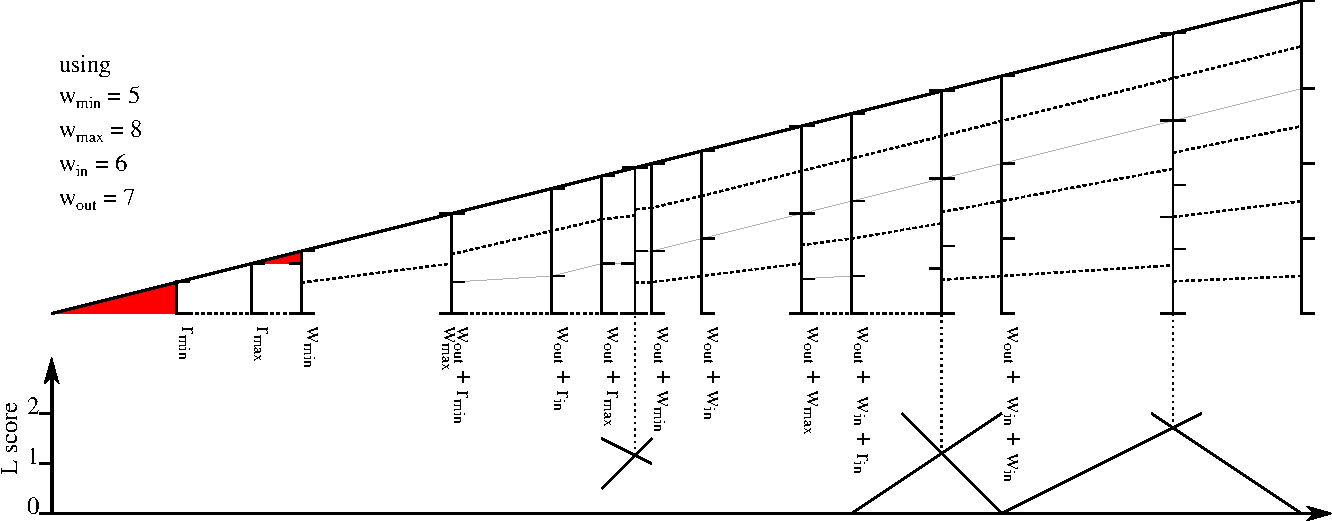
\includegraphics[width=.9\textwidth]{sources/method/ticking_v2.pdf}
\caption{Mapping of different lengths to a ticking. Transition location on a line-line segment is to the right of the middle because the preferred line width is to the left of the middle in the range.}
\label{transition_location}
\end{figure*}

We introduce a function which produces the $d$ at which all widths are prefered: 
\begin{align}
p(n) =
  \begin{cases} 
   \frac12 \wout & \text{if } n = \frac12 \\
    \wout + (n - 1) \win       & \text{otherwise}
  \end{cases}
\end{align}














\subsection{Skeletonization}
In order to apply the beading strategy to an arbitrary outline polygon we look at the skeleton of the polygon.
There are several possible skeletonal structures we could consider.


\subsubsection{Background}
One of the most commonly used skeletonizations of a shape is the medial axis.
The medial axis is defined by the locations where the inscribed circle meets the boundary in at least two locations. \todo{[citation needed]}
See \cref{MAT_explanation}.

``Because of its shape, the medial axis of a figure is also called the skeleton or the symmetric axis of the figure.
Associated with the medial axis is a radius function $R$, which defines for each point on the axis its distance to the boundary of the object.''
\cite{lee1982medial}

The medial axis along with the feature radius combine into a complete feature decsriptor, called the medial axis transform (MAT).
The MAT can unambiguously recreate the input shape exactly. \todo{[citation needed]}

\cite{Moesen2011} provides a thorough overview of all MAT algorithms.
\cite{Moesen2011} calls $R$ the `feature radius': ``In every point $p \in P$, and thus also in points on the MA, the feature radius $\text{rad}(p)$ of $p$ can be defined as the Euclidean distance to the closest point on the boundary of $P$.''


\begin{figure}
\centering
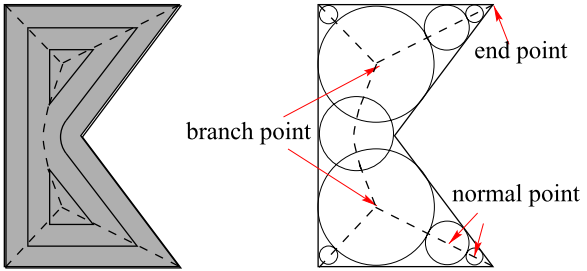
\includegraphics[width=.9\columnwidth]{sources/intro/medial_axis_Kao.png}
\caption{MAT explanation by \citeauthor{kao1998optimal}}
\label{MAT_explanation}
\end{figure}


\begin{figure}
\begin{subfigure}{0.3\columnwidth}
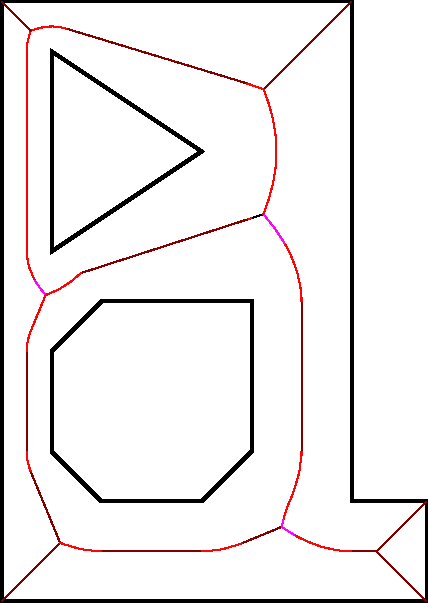
\includegraphics[width=\columnwidth]{sources/method/MAT_example.pdf}
\caption{MAT}
\end{subfigure}
\begin{subfigure}{0.3\columnwidth}
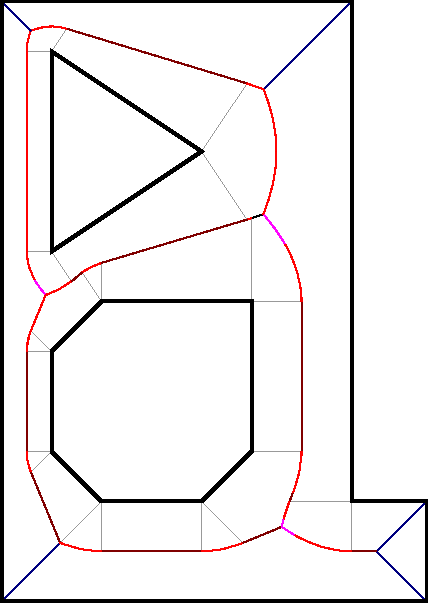
\includegraphics[width=\columnwidth]{sources/method/Voronoi_example.pdf}
\caption{Limited VD}
\end{subfigure}
\begin{subfigure}{0.3\columnwidth}
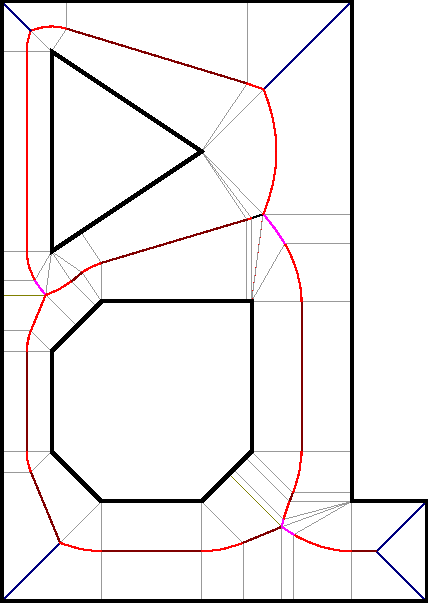
\includegraphics[width=\columnwidth]{sources/method/gMAT_example.pdf}
\caption{VQ}
\end{subfigure}
\caption{
Relation between the medial axis, the limited Voronoi Diagram and the Voronoi quadrangulation: MAT $\subset$ Limited VD $\subset$ VQ.
Significant parts of the skeleton are visualized in shades of red, insignificant regions in grey and blue.
}
\label{skeletonization_comparison}
\end{figure}



\subsubsection{Voronoi Quadrangulation}
The medial axis of a polygonal shape can be obtained from the Voronoi Diagram (VD) generated on the line segments and vertices of the shape. \cite{lee1982medial}
First we throw away all locations in the Voronoi diagram which fall outside the boundary shape.
We can then obtain the medial axis by further reducing the Voronoi bones connected to a concave corner in the boundary shape.

However, instead of removing bones from the Voronoi diagram we will introduce more bones such that the skeleton discretizes the boundary shape into quads within which the $R$ can be interpolated linearly.
We call the resulting skeletonization the \emph{Voronoi Quadrangulation} (VQ).
See \cref{skeletonization_comparison}.
The VQ greatly simplifies the processing required downstream in our framework.

In order to generate the VQ, we start by generating a normal Voronoi Diagram and remove all segments which lie outside of the boundary shape.
We then introduce bones such that each node in the VQ is directly connected to the outline via a single bone:
each node in the VQ is connected to the closest points on the boundary (its \emph{support}).
As such the VQ divides the polygon in quads consisting of 1 outline segment and 3 bones, one of which is not directly connected to the outline.
For concave verts the quad is missing the outline segments and so it regresses into a triangle;
likewise for convex sections it may happen that the inner bone is missing from the quad so that it forms a triangle.
\todo{TODO: make pics}

We then also discretize parabolic bones and bones generated by two concave outline vertices into approximately equidistant segments.
That way we can approximate the feature radius $R$ in between two nodes $v_0$ and $v_1$ in the VQ by interpolating linearly between $R(v_0)$ and $R(v_1)$.
Furthermore, we can linearly interpolate the distance field of a quad $p_0v_0v_1p_1$ (where $p_0$ and $p_1$ lie on the outline shape):
For a point $a \in p_0v_0$ and a point $b \in p_1v_1$ for which $R(a) = R(b)$ we have that all points in the line segment $ab$ have the same feature radius $R$.



\subsection{Beading}
We assign a bead count to each node in the skeleton which is connected to a bone which is in `the center' of the shape
and also to each node with locally optimal feature radius $R$.
Around regions where the bead count changes we introduce transition regions.


\subsubsection{Significance measure}\label{sec:significance_measure}
Places where the naive concentric toolpathing strategy would create large underfilling and overfilling areas are locations which intuitively look like `the center' of the shape.
This can be formalized by looking at the significance measure knows as the \emph{bisector angle}.
The bisector angle $\alpha$ is the angle $\widehat{p_ovp_1}$ between a location $v$ on a bone of the skeleton and its two supporting polygon points $p_0$ and $p_1$. \cite{attali1996modeling}
For a polygon with a pointy wedge area of an angle $\beta$, we have $\alpha = 180\degree - \beta$, which corresponds to overfill areas and underfill areas the size of $\nicefrac12 w^2 \left( \nicefrac14 \tan ( \alpha / 2) - \alpha / 2 \right)$ when filled using a naive strategy of constant bead width $w$.
See \cref{naive_overfill_underfill}.
The bisector angle is therefore an exact measure of the amount of overfill and underfill.
Contrary to related literature we will \emph{keep} the insignificant regions of the skeleton.
Our framework will employ a different toolpathing strategy to prevent overfill and underfill areas if they would be so large that $\alpha > \alpha_\text{max}$.


\begin{figure}
\centering
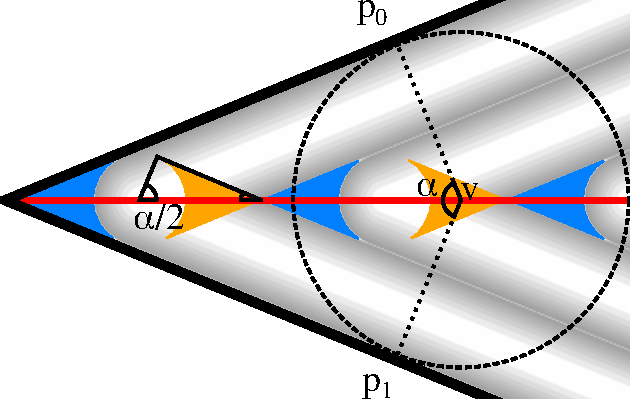
\includegraphics[width=\columnwidth]{sources/method/naive_overfill_underfill.pdf}
\caption{
Overfill and underfill areas in a naive beading using a constant bead witdh $w$ of a wedge area with vertex angle $\beta$.
The underfill areas (light blue) are mirrored versions of the overfill areas (dark red).
The bisector angle $a = 180\degree - \beta$ is the angle between a location $v$ and its support $p_0$ and $p_1$.
}
\label{naive_overfill_underfill}
\end{figure}


A computationally efficient way to compute $\alpha$ can be obtained by looking at the ratio between feature radius $R$ and the Euclidean distance.
if $ | R(v_1) - R(v_0) | / |v_1 - v_0| >  \sin(\alpha_\text{max} / 2)$ then $\alpha > \alpha_\text{max}$.
See \cref{distance_based_angles}.
This ratio can be immediately applied to simple skeleton segments to determine whether they are significant.
For skeletal segments generated by a polygon vertex and another vertex or line segment, we could exactly determine at which location $\frac{\partial R}{\partial x} > \sin(\alpha_\text{max} / 2)$.
However, because we have discretized such segments, we can approximate the location by applying our ratio based significance measure on the piecewise linear approximating segments directly.

\begin{figure}
\centering
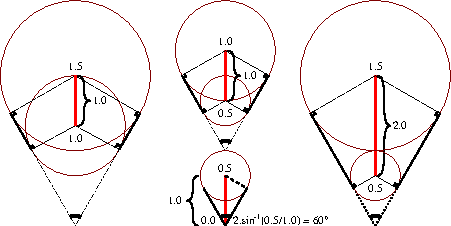
\includegraphics[width=.9\columnwidth]{sources/method/distance_based_angles.pdf}
\caption{Distance based angle estimation. By comparing the euclidean distance between two vertices with the distance measure of the MAT we can skip comparing the angles between the outline segments.}
\label{distance_based_angles}
\end{figure}

The Euclidean distance between two MAT vertices can never be less than the difference in the MAT distance measure between the vertices: \cref{distance_ratio_limit}.

\begin{figure}
\centering
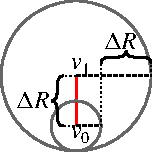
\includegraphics[width=.3\columnwidth]{sources/method/distance_ratio_limit.pdf}
\caption{Minimal Euclidean distance for a given difference in MAT distance measure.}
\label{distance_ratio_limit}
\end{figure}

Any node in the skeleton can have at most two significant bones connected to it, because we have limited $\alpha_\text{max} > 120\degree$,
while the corners of a triangle can only add up to \SI{180}{\degree}.
\todo{TODO: make figure which clearly shows this!}
This results in the fact that we will never have 3-way intersections of non-closed extrusion toolpaths.






\paragraph{Bead counts}
In order to apply the beading strategy to the VQ
we assign each significant node $v$ of the skeleton a bead count $v.B^*$ which is initialized to $b(R(v))$, but it is modified in order to prevent discontinuities and remaining gaps.

We also assign a bead count $v.B^*=b(R(v))$ to all nodes $v$ which are local maxima, i.e. the $v$ for which $\forall v_\text{n} \in v.\text{neighborhood} : R(v) > R(v_\text{n})$. 
This prevents the single overfill or underfill region in non-significant regions.
See \cref{rounded_vs_unrounded}.



\subsubsection{Transitioning}
In order to prevent discontinuities in the toolpaths around locations $p$ where $\exists n : R(p) = b^{-1}(n)$ (see \cref{transition_location}), we need a way to smoothly transition to a different number of beads around locations where the 3D model has a changing radius.
The transition will be placed so as to overlap the locations of $b^{-1}(n)$.

On the one side of the transition we will have $b^*(v_0)=\frac12 n$ and on the other side we will have $b^*(v_1)=\frac12 n + \frac12$.
For all locations on the MAT in between we linearly interpolate the $b^*$ values, so that we can later interpolate the bead widths $W$ linearly as well.



In a narrow wedge region (a.k.a. a cusp) we have to transfer from $n$ to $n+\nicefrac12$ beads; this transition requires a distance.
See \cref{single_bead_strategy_overview}.
The transition will be such that the innermost toolpath makes a \SI{45}{\degree} angle with the medial axis.
The length of the transition along the medial axis depends on the angles involved.
See \cref{transition_length}.
\begin{equation}
t = r_0 (\sin \alpha + \cos \alpha)
\end{equation}

\begin{figure}
\centering
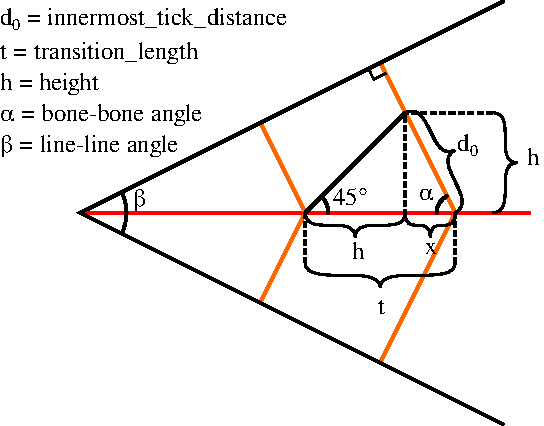
\includegraphics[width=.75\columnwidth]{sources/method/transition_length_v2.pdf}
\caption{Transition length on a line-line segment.}
\label{transition_length}
\end{figure}

The position of a transition should be at a location $p$ where $\exists n : R(p) = b^{-1}(n)$.
However, given the fact that a transition is a region rather than a point, which part of the transition should be ceneterd at $p$?
For a transition from $n$ to $n+\frac12$ beads, we place a fraction of the transition length toward the end with lower $R$ proportional to it's positioning within the region of non-prefered widths:
$ (b^{-1}(n+\frac12) - p(n) ) / (p(n + \frac12) - p(n))$
See \cref{transition_placement}.


\begin{figure}
\centering
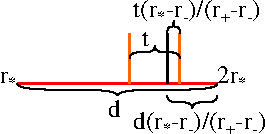
\includegraphics[width=.5\columnwidth]{sources/method/transition_location_precise.pdf}
\caption{Transition placement. The anchor position within the transition length is proportional to the transition location within the range between two distances with prefered length. \hl{outdated functions and variables!}}
\label{transition_placement}
\end{figure}

\hl{How to deal with non-marked regions shorter than the transition length?}


The transition needs to be robust against extra fingers in the MAT.
How do we compute the vertex location of an inset on a finger which crosses a transitioning area?
By interpolating the MAT distance between the two ends of the transition, we obtain a stable method for determining the vertex locations of insets.
See \cref{distance_rounding_transition}.
The extra fingers (blue) cause a negligible difference in the inset path (compare the black dashed pat hwith the red dashed path).
\hl{What does it look like for point-line segments or point-point segments?}

\begin{figure}
\centering
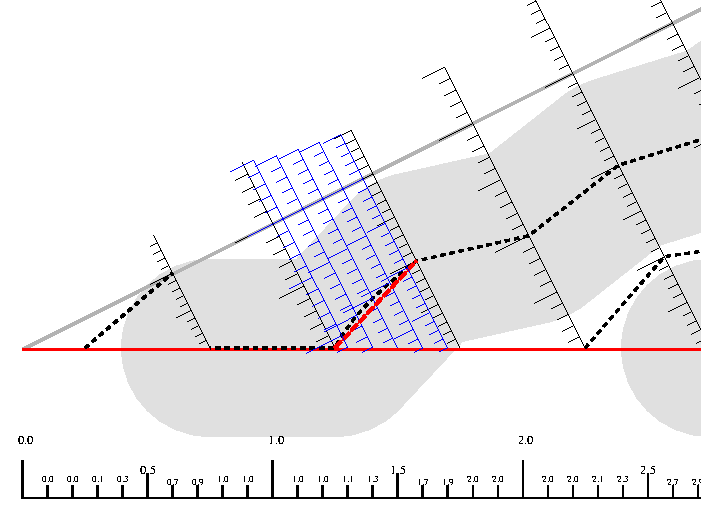
\includegraphics[width=.9\columnwidth]{sources/method/distance_rounding_transition.pdf}
\caption{MAT distance remapping.}
\label{distance_rounding_transition}
\end{figure}


\subsubsection{Ends of markings}
For vertices at the end of a sequence of marked MAT segments we need to take care of transitions.
If a transition is overlapping the end of the sequence, then either end of the transition would fall beyond the area where transitions should occur.
How should we deal with thse?
\begin{itemize}
\item We need to keep the transition tick on the marked side, because we need to switch to a different number of ticks somewhere.
Moreover, leaving out the whole transition around end-of-markings would violate the stability principle.
\item The end-of-marking itself will retain its interpolated MAT distance as described above.
\item The transition tick on the non-marked side of discarded.
This means that there will also be no single bead segment leading up to the transition, which coincides with how we deal with non-marked areas.
See \cref{single_bead_strategy}.
\end{itemize}
This method of dealing with end-of-markings can result in gaps slightly larger than usual.
See \cref{change_to_marked}.

\begin{figure}
\begin{subfigure}{0.45\columnwidth}
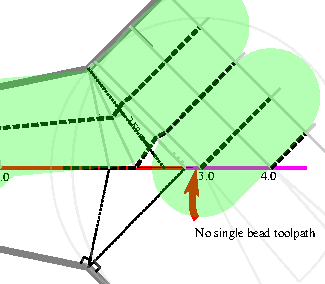
\includegraphics[width=\columnwidth]{sources/method/change_to_marked.pdf}
\caption{before end of markings}
\end{subfigure}
\begin{subfigure}{0.45\columnwidth}
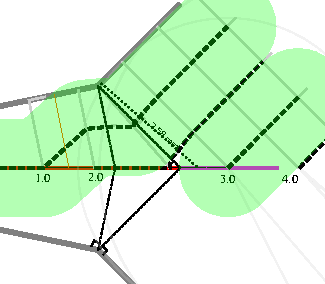
\includegraphics[width=\columnwidth]{sources/method/change_to_marked_2.pdf}
\caption{after end of markings}
\end{subfigure}
\caption{Transition near end of markings. The gap depends on the positioning of the middle of the transition (dotted lines) with respect to the end of the marked areas.}
\label{change_to_marked}
\end{figure}


It impossible for three marked edges to come together.
(Simple case) If 2 edges of the MAT meet then 3 outline segments are involved; lines through those segments form a triangle which cannot have more than two angles less than \SI{60}{\degree}.
However, what if we connect two marked segments using a small non-marked segment?
There is a distance limit based on \cref{distance_ratio_limit}:
the connecting segment is always larger in Euclidean distance than the difference in MAT distance.




\subsubsection{Introduce joints at transition ends}
At the locations $v$ of prefered width, i.e. when $R(v) = p(b(R(v)))$.
We discretize the distance measure field piecewise linear.
In \cref{distance_rounding_transition} we have one piece at MAT dist $0.0$ from bar $0$ to bar $2.5$, than a piece increasing from MAT dist $0.0$ to $1.0$ from bar $2.5$ to $7.5$ etc.

At the end of a marked section we round the MAT distance measure to the nearest integer and introduce a joint there and connect it to the outline using a new finger.
At those places we round the distance measure without applying transitioning, because the end of the transition would lie beyond the marked region.
 
\paragraph{Note}
We could introduce bones implicitly.
Instead of changing the straight skeleton and introducing bones,
we can simply introduce new vertices on the polygon and generate a new straight skeleton.

\old{
One could think that this means that the method for introducing joints in the original medial axis should be the same method as used for introducing joints on the newly added fingers connected to the joints introduced in the first step!
}
However, the method for introducing joints on the marked regions may differ from the method for introducing joints on the non-marked regions!




\subsection{Toolpath extraction}

\subsubsection{Tick placement}
\hl{Change terminology: location $\to$ junction?}

Now that we have the skeleton set up, we determine the locations along the bones where the vertices of the toolpath polygons should be.
For marked regions / significant regions we have already inroduced joints around the transitions which serve as those locations.
For non-marked regions / unsignificant regions we can simply apply the beading strategy in order to find the toolpath verts.


This needs to be stable against small perturbations in the outline polygon.
See \cref{heterogeneous_joint_generation}.
For any sequence on non-marked bones from the outline polygon inward we define the stable end point as the first vertex which is connected to a marked medial axis segment.
Based on the MAT distance $R$ there we place ticks along the non-marked bones following the beading strategy.

\begin{figure}
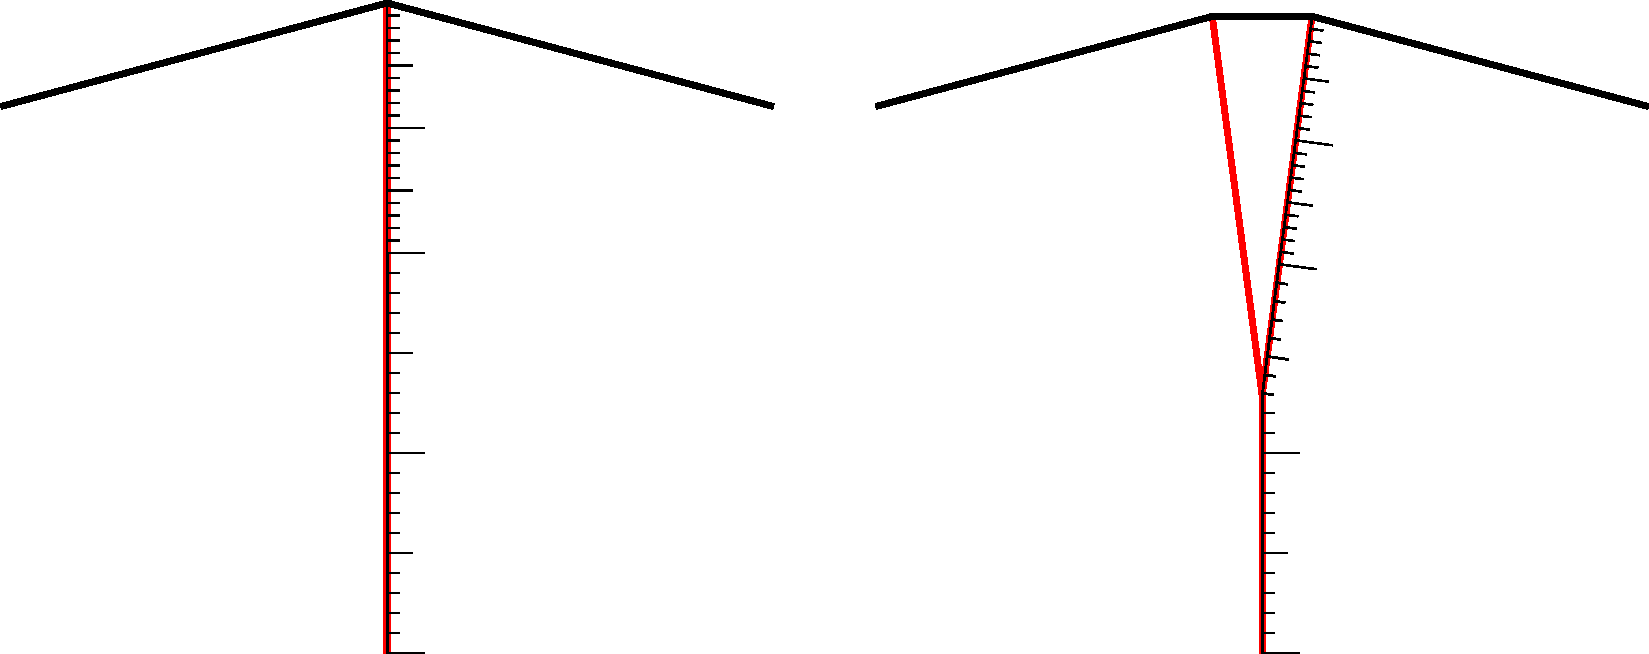
\includegraphics[width=\columnwidth]{sources/method/heterogeneous_joint_generation.pdf}
\caption{Toolpaths employing dist rounding vs without.}
\label{heterogeneous_joint_generation}
\end{figure}





\subsubsection{Toolpath extraction algorithm}
After the beading strategy has been applied we have a beading associated with each significant node as well as each node with locally optimal $R$.
In order to determine the tick locations of quads which don't contain any such node, we propagate the beading information down.
We therefore sort all quads on their highest $R$-value and process the high $R$ quads first.
The beading information is then passed down along the bones of the quad to lower $R$ nodes if those nodes don't already have a beading associated.

See \cref{alg_beading_propagation}.

\begin{algorithm}
\caption{Beading propagation}
\label{alg_beading_propagation}
\begin{algorithmic}
\State quads.sortOn(getHighestR())
\ForAll{$q \in$ quads}
	\State $v_\text{max} = q$.getHighestR()
	\State beading = retrieveBeading($v_\text{max}$)
	\If {$\neg$ retrieveBeading($v_\text{max}$.next())}
		\State storeBeading($v_\text{max}$.next(), beading)
	\EndIf
	\If {$\neg$ retrieveBeading($v_\text{max}$.prev())}
		\State storeBeading($v_\text{max}$.prev(), beading)
	\EndIf
\EndFor
\end{algorithmic}
\end{algorithm}


We can then process all bones in arbitrary order and generate the ticks along those bones.
See \cref{alg_tick_generation}.

\begin{algorithm}
\caption{Tick generation}
\label{alg_tick_generation}
\lstset{language=C++}
\begin{lstlisting}[frame=single]
Point a = edge->to->p;
Point b = edge->from->p;
Point ab = b - a;

int start_R = edge->to->data.distance_to_boundary; // higher R
int end_R = edge->from->data.distance_to_boundary; // lower R
assert(end_R <= start_R);

int junction_idx;
// compute starting junction_idx for this segment
for (junction_idx = (beading->toolpath_locations.size() - 1) / 2; junction_idx >= 0 && junction_idx < beading->toolpath_locations.size(); junction_idx--)
{
  int bead_R = beading->toolpath_locations[junction_idx];
  if (bead_R <= start_R)
    break; // junction coinciding with start node is used in this function call
}

for (; junction_idx >= 0 && junction_idx < coord_t(beading->toolpath_locations.size()); junction_idx--)
{
  int bead_R = beading->toolpath_locations[junction_idx];
  assert(bead_R > 0);
  if (bead_R < end_R)
    break; // junction coinciding with a node is handled by the next segment
  
  Point junction(a + ab * (bead_R - start_R) / (end_R - start_R));
  ticks.emplace_back(junction, beading->bead_widths[junction_idx], junction_idx);
}
\end{lstlisting}
\end{algorithm}


We then generate bead segments for each quad by connecting together the ticks of the same index.
If the amount of ticks on both sides of the quad is not the same then this quad is in a transition and we leave one tick unconnected.


\paragraph{Printing order}
The order in which beads are printed has influence on the quality and dimensional accuracy of a print.
If the inner beads are printed first then small inaccuracies in the deposition process propagate outward and the final outline of the print layer will be less accurate.
However, if the second bead is printed before the outer bead then the outer bead has more material to adhere to, which lessens the overhang constraints.
We therefore choose to print the inner beads first starting from the second bead and at the very end print the outermost bead.


When all extrusion segments are generated, we combine them into semi-continuous polyline toolpaths.
These polylines generally form closed polygons, but at significant regions of the VQ the toolpaths consist of single bead polyline toolpaths.
See \cref{single_bead_strategy}.
These single bead polylines can connect to polygonal toolpaths and they can also meet each other at 3-way junctions.
We determine the printing order for all segments of a given bead index by minimizing the travel distance using a greedy path order optimizer.
\todo{[implementation needed!]}


In general the toolpath location should be centered on the middle of the bead.
However, when the bead width is smaller than the nozzle size we might want to offset the toolpath toward a previously printed bead.
That way the previously printed bead occludes part of the hole in the nozzle such that the unoccluded hole is as wide as the required bead width.
The printing order and the toolpath positioning of the beading strategy are therefore interrelated.

Around 3-way junctions we need to prevent overextrusion.
We need to reduce the extrusion amount after the first time we pass an intersection: commonly known as \emph{ghosting}.
See \cref{ghosting}.
In order to realize the reduction we remove a section from the extrusion bead up to a distance equal to the feature radius from the junction.


\begin{figure}
\centering
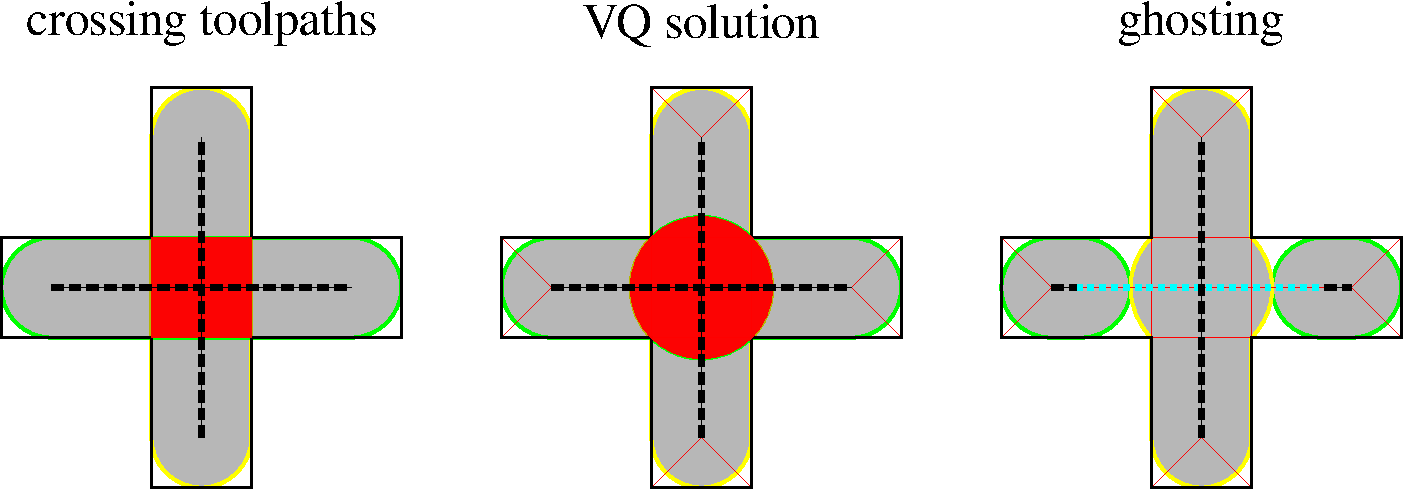
\includegraphics[width=.99\columnwidth]{sources/method/ghosting.pdf}
\caption{Ghosting prevents over-extrusion at junctions.}
\label{ghosting}
\end{figure}


























































